\documentclass[12pt]{article}
\usepackage{fullpage}
\usepackage{pgf,tikz}
\usepackage{mathrsfs}
\usetikzlibrary{arrows}
\newcommand{\degre}{\ensuremath{^\circ}}
\title{Angles and Triangles}
\author{Grade 5-6 Olympic Math}
\date{January 9, 2016}
\begin{document}
	\maketitle
	\begin{enumerate}
		\item In the following figures, find the angles denoted by the question marks.
		
		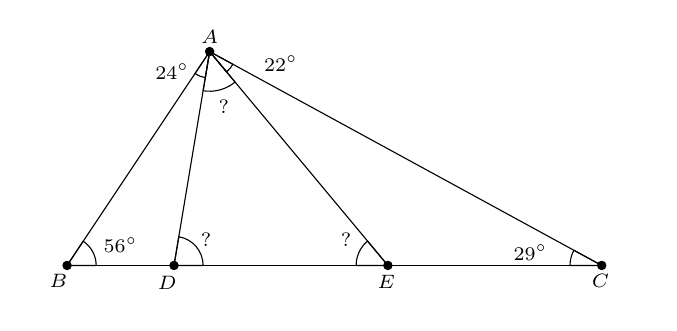
\begin{tikzpicture}[line cap=round,line join=round,>=triangle 45,x=0.452679802594599125cm,y=0.452679802594599125cm]
		\clip(12.8948188000025,-10.075869337229813) rectangle (30.332031688779924,-2.344134941440011);
		\fill[fill=white](18.,-3.0148401811819383) -- (14.,-9.014840181181938) -- (29.,-9.014840181181938) -- cycle;
		\fill[fill=white](18.,-3.0148401811819383) -- (17.,-9.014840181181938) -- (23.,-9.014840181181938) -- cycle;
		\draw [shift={(18.,-3.0148401811819383)}] (0,0) -- (-123.6900675259798:0.7420090590969116) arc (-123.6900675259798:-99.46232220802563:0.7420090590969116) -- cycle;
		\draw [shift={(14.,-9.014840181181938)}] (0,0) -- (0.:0.8162099650066027) arc (0.:56.309932474020215:0.8162099650066027) -- cycle;
		\draw [shift={(18.,-3.0148401811819383)}] (0,0) -- (-50.19442890773481:0.7420090590969116) arc (-50.19442890773481:-28.61045966596522:0.7420090590969116) -- cycle;
		\draw [shift={(29.,-9.014840181181938)}] (0,0) -- (151.3895403340348:0.8904108709162939) arc (151.3895403340348:180.:0.8904108709162939) -- cycle;
		\draw [shift={(18.,-3.0148401811819383)}] (0,0) -- (-99.46232220802563:1.1130135886453674) arc (-99.46232220802563:-50.19442890773481:1.1130135886453674) -- cycle;
		\draw [shift={(17.,-9.014840181181938)}] (0,0) -- (0.:0.8162099650066027) arc (0.:80.53767779197439:0.8162099650066027) -- cycle;
		\draw [shift={(23.,-9.014840181181938)}] (0,0) -- (129.8055710922652:0.8904108709162939) arc (129.8055710922652:180.:0.8904108709162939) -- cycle;
		\draw (18.,-3.0148401811819383)-- (14.,-9.014840181181938);
		\draw (14.,-9.014840181181938)-- (29.,-9.014840181181938);
		\draw (29.,-9.014840181181938)-- (18.,-3.0148401811819383);
		\draw (18.,-3.0148401811819383)-- (17.,-9.014840181181938);
		\draw (17.,-9.014840181181938)-- (23.,-9.014840181181938);
		\draw (23.,-9.014840181181938)-- (18.,-3.0148401811819383);
		\begin{scriptsize}
		\draw [fill=black] (18.,-3.0148401811819383) circle (1.5pt);
		\draw[color=black] (17.999841126589253,-2.6) node {$A$};
		\draw [fill=black] (14.,-9.014840181181938) circle (1.5pt);
		\draw[color=black] (13.755549308554917,-9.43774154640647) node {$B$};
		\draw [fill=black] (29.,-9.014840181181938) circle (1.5pt);
		\draw[color=black] (28.966735020041607,-9.452581727588408) node {$C$};
		\draw [fill=black] (17.,-9.014840181181938) circle (1.5pt);
		\draw[color=black] (16.812626632034195,-9.497102271134223) node {$D$};
		\draw [fill=black] (23.,-9.014840181181938) circle (1.5pt);
		\draw[color=black] (22.956461641356622,-9.482262089952284) node {$E$};
		\draw[color=black] (16.94618826267164,-3.575869979540882) node {$24\textrm{\degre}$};
		\draw[color=black] (15.5,-8.44344940721661) node {$56\textrm{\degre}$};
		\draw[color=black] (20,-3.353267261811809) node {$22\textrm{\degre}$};
		\draw[color=black] (27,-8.65) node {$29\textrm{\degre}$};
		\draw[color=black] (18.4,-4.5701621187307415) node {?};
		\draw[color=black] (17.9,-8.3) node {?};
		\draw[color=black] (21.828607871529318,-8.3) node {?};
		\end{scriptsize}
		\end{tikzpicture}
		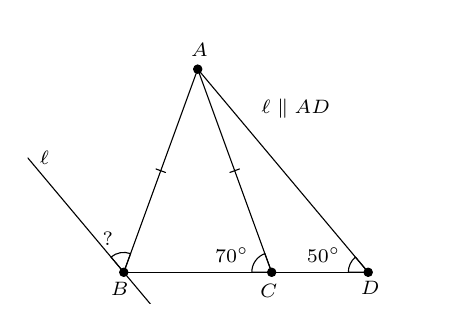
\begin{tikzpicture}[line cap=round,line join=round,>=triangle 45,x=0.68638790849047125cm,y=0.68638790849047125cm]
		\clip(17.22193647303614,-15.573314486792855) rectangle (24.51520250156249,-10.47415706180656);
		\draw [shift={(23.522063499388548,-15.)}] (0,0) -- (130.:0.3677276989172951) arc (130.:180.:0.3677276989172951) -- cycle;
		\draw [shift={(21.736161146605347,-15.)}] (0,0) -- (110.:0.3677276989172951) arc (110.:180.:0.3677276989172951) -- cycle;
		\draw [shift={(19.,-15.)}] (0,0) -- (70.:0.3677276989172951) arc (70.:130.:0.3677276989172951) -- cycle;
		\draw [domain=17.22193647303614:24.51520250156249] plot(\x,{(--295.47125082498223-46.07016386514917*\x)/38.65745750752346});
		\draw (19.,-15.)-- (20.368080573302674,-11.24122951685636);
		\draw (19.595939337975032,-13.088548635499393) -- (19.772141235327638,-13.152680881356964);
		\draw (21.736161146605347,-15.)-- (19.,-15.);
		\draw (20.368080573302674,-11.24122951685636)-- (21.736161146605347,-15.);
		\draw (21.14022180863031,-13.088548635499393) -- (20.96401991127771,-13.152680881356964);
		\draw (20.368080573302674,-11.24122951685636)-- (23.522063499388548,-15.);
		\draw (23.522063499388548,-15.)-- (21.736161146605347,-15.);
		\begin{scriptsize}
		\draw (17.3,-12.606977715526789) node[anchor=north west] {$\ell$};
		\draw (21.401774650729394,-11.65088569834186) node[anchor=north west] {$\ell\parallel AD$};
		\draw [fill=black] (21.736161146605347,-15.) circle (1.5pt);
		\draw[color=black] (21.68369921989932,-15.340420277478575) node {$C$};
		\draw [fill=black] (20.368080573302674,-11.24122951685636) circle (1.5pt);
		\draw[color=black] (20.4,-10.89) node {$A$};
		\draw [fill=black] (23.522063499388548,-15.) circle (1.5pt);
		\draw[color=black] (23.559110484377527,-15.291389917622938) node {$D$};
		\draw[color=black] (22.7,-14.67851041942747) node {$50\textrm{\degre}$};
		\draw [fill=black] (19.,-15.) circle (1.5pt);
		\draw[color=black] (18.925741478019606,-15.315905097550758) node {$B$};
		\draw[color=black] (21,-14.67851041942747) node {$70\textrm{\degre}$};
		\draw[color=black] (18.70510485866923,-14.372070670329737) node {?};
		\end{scriptsize}
		\end{tikzpicture}
		
		\begin{tikzpicture}[line cap=round,line join=round,>=triangle 45,x=0.47581180324552971428571428571429cm,y=0.47581180324552971428571428571429cm]
		\clip(11.203673096541811,-12.252029402771534) rectangle (22.484902143131876,-3.8453442959375845);
		\draw [shift={(19.,-7.)}] (0,0) -- (0.:0.6327612446004043) arc (0.:112.5:0.6327612446004043) -- cycle;
		\draw(12.,-7.383511228796273) -- (12.383511228796273,-7.383511228796273) -- (12.383511228796273,-7.) -- (12.,-7.) -- cycle; 
		\draw(15.616488771203727,-7.) -- (15.616488771203727,-7.383511228796273) -- (16.,-7.383511228796273) -- (16.,-7.) -- cycle; 
		\draw(16.,-10.616488771203727) -- (15.616488771203727,-10.616488771203727) -- (15.616488771203727,-11.) -- (16.,-11.) -- cycle; 
		\draw(12.383511228796273,-11.) -- (12.383511228796273,-10.616488771203727) -- (12.,-10.616488771203727) -- (12.,-11.) -- cycle; 
		\draw (12.,-7.)-- (12.,-11.);
		\draw (12.19540743175704,-9.) -- (11.804592568242953,-9.);
		\draw (12.,-11.)-- (16.,-11.);
		\draw (14.,-10.804592568242958) -- (14.,-11.19540743175704);
		\draw (16.,-11.)-- (16.,-7.);
		\draw (15.804592568242954,-9.) -- (16.195407431757044,-9.);
		\draw (16.,-7.)-- (12.,-7.);
		\draw (14.,-7.195407431757041) -- (14.,-6.804592568242958);
		\draw (12.,-11.)-- (16.,-7.);
		\draw (16.,-7.)-- (19.,-7.);
		\draw (17.46836193776998,-6.91864498283709) -- (17.46836193776998,-7.081355017162909);
		\draw (17.53163806223002,-6.91864498283709) -- (17.53163806223002,-7.081355017162909);
		\draw (19.,-7.)-- (22.,-7.);
		\draw (18.121320343559642,-4.878679656440358)-- (19.,-7.);
		\draw (16.,-7.)-- (18.121320343559642,-4.878679656440358);
		\draw (16.98076199911393,-5.904184632247187) -- (17.095815367752813,-6.019238000886068);
		\draw (17.02550497580683,-5.859441655554289) -- (17.14055834444571,-5.97449502419317);
		\begin{scriptsize}
		\draw [fill=black] (12.,-7.) circle (1.5pt);
		\draw[color=black] (11.854513233845083,-6.304073703527729) node {$A$};
		\draw [fill=black] (12.,-11.) circle (1.5pt);
		\draw[color=black] (11.854513233845083,-11.637347050873998) node {$B$};
		\draw [fill=black] (16.,-11.) circle (1.5pt);
		\draw[color=black] (15.795711843070459,-11.565031480062522) node {$C$};
		\draw [fill=black] (16.,-7.) circle (1.5pt);
		\draw[color=black] (15.397976203607346,-6.4306259524478095) node {$D$};
		\draw [fill=black] (19.,-7.) circle (1.5pt);
		\draw[color=black] (18.851044709855266,-7.587675085431407) node {$E$};
		\draw [fill=black] (18.121320343559642,-4.878679656440358) circle (1.5pt);
		\draw[color=black] (18.037494538226177,-4.405789969726515) node {$F$};
		\draw[color=black] (19.375332598238458,-5.9244169567674865) node {?};
		\end{scriptsize}
		\end{tikzpicture}
		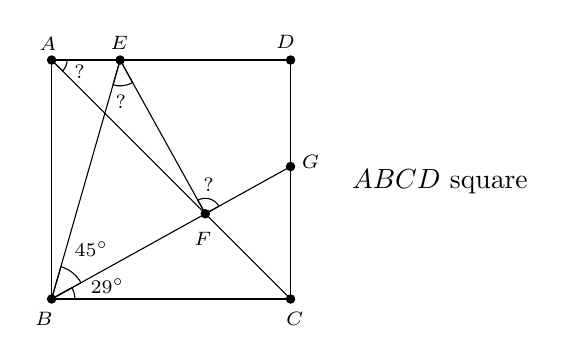
\begin{tikzpicture}[line cap=round,line join=round,>=triangle 45,x=0.50578154271900662857142857142857cm,y=0.50578154271900662857142857142857cm]
		\draw [shift={(17.,-7.)}] (0,0) -- (0.:0.5834178242780433) arc (0.:29.:0.5834178242780433) -- cycle;
		\draw [shift={(17.,-7.)}] (0,0) -- (29.:0.8427146350682848) arc (29.:74.:0.8427146350682848) -- cycle;
		\draw [shift={(20.86023615727642,-4.860236157276422)}] (0,0) -- (29.:0.3889452161853622) arc (29.:119.:0.3889452161853622) -- cycle;
		\draw [shift={(18.72047231455285,-1.)}] (0,0) -- (-106.:0.6482420269756037) arc (-106.:-61.:0.6482420269756037) -- cycle;
		\draw [shift={(17.,-1.)}] (0,0) -- (-45.:0.3889452161853622) arc (-45.:0.:0.3889452161853622) -- cycle;
		\draw (17.,-1.)-- (17.,-7.);
		\draw (17.,-7.)-- (23.,-7.);
		\draw (23.,-7.)-- (23.,-1.);
		\draw (23.,-1.)-- (17.,-1.);
		\draw (17.,-1.)-- (23.,-7.);
		\draw (18.72047231455285,-1.)-- (20.86023615727642,-4.860236157276422);
		\draw (18.72047231455285,-1.)-- (17.,-7.);
		\draw (23.,-3.6741456912833836)-- (17.,-7.);
		\draw (24.298958725037068,-3.5) node[anchor=north west] {$ABCD$ square};
		\begin{scriptsize}
		\draw [fill=black] (17.,-1.) circle (1.5pt);
		\draw[color=black] (16.90899961751519,-0.6031032246837088) node {$A$};
		\draw [fill=black] (17.,-7.) circle (1.5pt);
		\draw[color=black] (16.805280893199093,-7.5) node {$B$};
		\draw [fill=black] (23.,-7.) circle (1.5pt);
		\draw[color=black] (23.10619339540196,-7.5) node {$C$};
		\draw [fill=black] (23.,-1.) circle (1.5pt);
		\draw[color=black] (22.872826265690744,-0.5382790219861485) node {$D$};
		\draw[color=black] (18.4,-6.68) node {$29\textrm{\degre}$};
		\draw[color=black] (18,-5.75) node {$45\textrm{\degre}$};
		\draw [fill=black] (18.72047231455285,-1.) circle (1.5pt);
		\draw[color=black] (18.698147611967855,-0.5642087030651727) node {$E$};
		\draw [fill=black] (20.86023615727642,-4.860236157276422) circle (1.5pt);
		\draw[color=black] (20.8,-5.5) node {$F$};
		\draw [fill=black] (23.,-3.6741456912833836) circle (1.5pt);
		\draw[color=black] (23.5,-3.5461220271529466) node {$G$};
		\draw[color=black] (20.941065025303445,-4.142504691970502) node {?};
		\draw[color=black] (18.737042133586392,-2.0422005245695476) node {?};
		\draw[color=black] (17.7,-1.3032046138173603) node {?};
		\end{scriptsize}
		\end{tikzpicture}
		
		\item What is the maximum number of acute interior angles a triangle can have? Right angles? Obtuse angles?
		
		\item \begin{enumerate}
			\item What is the sum of the interior angles of a quadrilateral?
			
			\item What is the sum of the interior angles of an $n$-gon (a polygon with $n$ sides)?
		\end{enumerate}
		
		\item Let $ABC$ be a triangle and suppose that there is a point $D$ on $BC$ such that $AD=BD=CD$. Show that $\angle BAC = 90\degre$.
		
		\item Let $ABC$ be a right angle triangle with hypotenuse $BC$, and let $D$ be the midpoint of $BC$. Show that $AD=BD=CD$.
		
		(\emph{Hint:} Let $D'$ be the point on $BC$ such that $AD'=BD'$. Show that $AD'=CD'$ by angle chasing.)
	\end{enumerate}
\end{document}